\documentclass[compress]{beamer}
\usepackage{ifthen,verbatim}

\newcommand{\isnote}{}
\xdefinecolor{lightyellow}{rgb}{1.,1.,0.25}
\xdefinecolor{darkblue}{rgb}{0.1,0.1,0.7}

%% Uncomment this to get annotations
%% \def\notes{\addtocounter{page}{-1}
%%            \renewcommand{\isnote}{*}
%% 	   \beamertemplateshadingbackground{lightyellow}{white}
%%            \begin{frame}
%%            \frametitle{Notes for the previous page (page \insertpagenumber)}
%%            \itemize}
%% \def\endnotes{\enditemize
%% 	      \end{frame}
%%               \beamertemplateshadingbackground{white}{white}
%%               \renewcommand{\isnote}{}}

%% Uncomment this to not get annotations
\def\notes{\comment}
\def\endnotes{\endcomment}

\setbeamertemplate{navigation symbols}{}
\setbeamertemplate{headline}{\mbox{ } \hfill
\begin{minipage}{5.5 cm}
\vspace{-0.75 cm} \small
\end{minipage} \hfill
\begin{minipage}{4.5 cm}
\vspace{-0.75 cm} \small
\begin{flushright}
\ifthenelse{\equal{\insertpagenumber}{1}}{}{Jim Pivarski \hspace{0.2 cm} \insertpagenumber\isnote/\pageref{numpages}}
\end{flushright}
\end{minipage}\mbox{\hspace{0.2 cm}}\includegraphics[height=1 cm]{../cmslogo} \hspace{0.1 cm} \includegraphics[height=1 cm]{../tamulogo} \hspace{0.01 cm} \vspace{-1.05 cm}}

\begin{document}
\begin{frame}
\vfill
\begin{center}
\textcolor{darkblue}{\Large HIP/MP Comparisons and HIP Results}

\vfill
\begin{columns}
\column{0.3\linewidth}
\begin{center}
\large
\textcolor{darkblue}{Jim Pivarski}

\vspace{0.2 cm}
Alexei Safonov
\end{center}
\end{columns}

\begin{columns}
\column{0.3\linewidth}
\begin{center}
\scriptsize
{\it Texas A\&M University}
\end{center}
\end{columns}

\vfill
25 May, 2009

\end{center}
\end{frame}

%% \begin{notes}
%% \item This is the annotated version of my talk.
%% \item If you want the version that I am presenting, download the one
%% labeled ``slides'' on Indico (or just ignore these yellow pages).
%% \item The annotated version is provided for extra detail and a written
%% record of comments that I intend to make orally.
%% \item Yellow notes refer to the content on the {\it previous} page.
%% \item All other slides are identical for the two versions.
%% \end{notes}

\small

\begin{frame}
\frametitle{Agreement on an alignment?}

\begin{itemize}\setlength{\itemsep}{0.1 cm}
\item Pablo and I discussed implementation details  early in the week
\item We synchronized all of the inputs and many of the
  parameters/cuts, and set up parallel CRAFT alignments and tests in
  cosmic ray MC
\item We didn't finish our comparison--- I have not seen all of the
  MP results--- and we never got a chance to discuss how we might
  converge (schedule conflicts? a bad week?)
\item What I know is the following:
\begin{itemize}\setlength{\itemsep}{0.1 cm}
\item even with the same inputs and similar cuts, HIP and MP differ in
  data by 2--4~mm, 0.5--2~mrad, systematic trend in $y$, $z$
\item HIP yields high-accuracy results in Monte Carlo
\end{itemize}
\item What I'll present here:
\begin{itemize}
\item comparative study of HIP and MP implementations and results
\item possible explanations for the discrepancy
\item my HIP recommendation, and arguments to support it as a good sub-millimeter alignment
\end{itemize}
\end{itemize}
\end{frame}

%% \begin{frame}
%% \frametitle{Outline}
%% \begin{itemize}\setlength{\itemsep}{0.15 cm}
%% \item Comparison of results from HIP and MillePede implementations
%% \begin{itemize}
%% \item synchronized cuts/inputs: incidental differences that could be made the same were made the same
%% \item Alicia's verification with segments
%% \end{itemize}

%% \item Comparison of the algorithms
%% \begin{itemize}
%% \item motivations for remaining differences
%% \item cosmic ray Monte Carlo test to diagnose differences
%% \end{itemize}

%% \item Proposed constants for re-processing
%% \begin{itemize}
%% \item differences with respect to CRAFT\_ALL\_V11
%% \end{itemize}

%% \item Systematic effects that we don't understand
%% \begin{itemize}
%% \item sawtooth
%% \item $p_T$ dependence
%% \item internal structure in station 4
%% \end{itemize}

%% \item Work toward producing a CSC disk alignment by the end of \mbox{the week\hspace{-1 cm}}
%% \end{itemize}
%% \end{frame}

\begin{frame}
\frametitle{Comparison of HIP and MP (1/3)}
\begin{itemize}
\item Inputs to the procedures \textcolor{darkblue}{\scriptsize (differences between HIP and MP in blue)}
\begin{itemize}\setlength{\itemsep}{0.1 cm}\scriptsize
\item {\tiny V11\_StreamMuAlGlobalCosmics\_227\_Tosca090216\_FromTrackerPointing\_v5} \mbox{(RunReg 3.8~T only)\hspace{-1 cm}}
\item newest tracker alignment (c.~May 19)
\item last month's tracker APEs (c.~Apr 24): update not available
\item tracker hits $\ge$ 15, $\chi^2/N_{\mbox{\scriptsize dof}}$ $<$ 10, TIB and TOB only
\item high momentum: $100 < p_T < 200$~GeV
\item latest magnetic field: ``grid\_1103l\_090322\_3\_8t''
\item latest internal DT alignment \mbox{(agreement between tracks and survey)\hspace{-1 cm}}
\item \textcolor{darkblue}{HIP: CMSSW\_2\_2\_11, MP: CMSSW\_2\_2\_10} {\it (very likely no difference for

\hfill our purposes)}
\end{itemize}
\end{itemize}

\vspace{-0.35 cm}
\begin{columns}
\column{0.57\linewidth}
\includegraphics[height=\linewidth, angle=90]{SuperHIPMPmerged_TrackChi2n.pdf}
\column{0.45\linewidth}
\begin{itemize}\setlength{\itemsep}{-0.05 cm}\scriptsize
\item Newest tracker alignment is the light blue one
\item New $\chi^2/N_{\mbox{\scriptsize dof}}$ peaks at 1.4 without APEs, old peaks at 1.6
\item Tracker alignment still needs to be centered and APEs need to be produced

Final muon alignment will need to be consistent with final tracker alignment
\end{itemize}
\end{columns}
\end{frame}

\begin{frame}
\frametitle{Comparison of HIP and MP (2/3)}
\begin{itemize}\setlength{\itemsep}{0.25 cm}
\item Alignables/parameters \textcolor{darkblue}{\scriptsize (differences between HIP and MP in blue)}
\begin{itemize}\setlength{\itemsep}{0.1 cm}\scriptsize
\item only wheels $-$1, 0, $+$1, all sectors except 1 and 7
\item stations 1--3: 6 degrees of freedom
\item station 4: \textcolor{darkblue}{HIP: $x$, $\phi_y$, $\phi_z$, MP: $x$, $\phi_y$} {\it (we'll compare only stations 1--3)}
\end{itemize}

\item Algorithmic implementation
\begin{itemize}\setlength{\itemsep}{0.1 cm}\scriptsize
\item no treatment of $\vec{B}$-field, $dE/dx$ effects (HIP and MP implementations differ, so we turned them both off; note that $p_T > 100$~GeV)
\item residuals calculated from standard CMSSW track-refits with muon chamber APEs $\to$ $\infty$ (1000~cm)
\item segment residuals: \textcolor{darkblue}{HIP: linear fit to (extrapolated track $-$ hits), \\ MP: (extrapolated track) $-$ (linear fit to hits)} \mbox{\it (negligible: $\vec{B} \approx 0$ inside DTs)\hspace{-1 cm}}
\item cut on muon residuals: \textcolor{darkblue}{HIP: keep residuals tails \mbox{(cut only unphysical values),\hspace{-1 cm}} \\ MP: cut $1 \, \sigma$ symmetrically around the peak}
\item treatment of residuals tails: \textcolor{darkblue}{HIP: fit tail shape and \mbox{misalignment together,\hspace{-1 cm}} \\ MP: calculate misalignment from matrix inversion of hits}
\item residuals weights: HIP: segment residual $(\chi^2/N_{\mbox{\scriptsize dof}})^{-1}$, MP: \textcolor{darkblue}{the same?}
\item iteration: \textcolor{darkblue}{HIP: 2 required, 3 applied, MP: 1 applied}
\end{itemize}
\end{itemize}

We'll discuss the algorithmic differences soon
\end{frame}

\begin{frame}
\frametitle{Comparison of HIP and MP (3/3)}

\begin{itemize}\scriptsize
\item Absolute differences (MP $-$ HIP) on the order of \mbox{0.5--2.5~mm, 0.5--2~mrad\hspace{-1 cm}}
\item In this comparison, station 4 is excluded, as are \mbox{3 failed fits {\scriptsize (too few hits)}:\hspace{-1 cm}}

\mbox{ } \hfill wh$-$1, st2, sec08 \hfill wh$+$1, st2, sec02 \hfill wh$+$1, st3, sec08 \hfill \mbox{ }

\item Orientation of local $x$, $y$, $z$ directions are ideal \mbox{{\scriptsize (for symmetric comparison)}:\hspace{-1 cm}}
\end{itemize}

\vfill \only<1>{\includegraphics[height=\linewidth, angle=90]{hip_millepede_difference.pdf}}\only<2>{\includegraphics[height=\linewidth, angle=90]{hip_millepede_difference2.pdf}}

\tiny \textcolor{red}{This plot now uses the latest tracker for both HIP and MillePede!}
\end{frame}

\begin{frame}
\frametitle{Implementation details}
\begin{itemize}\setlength{\itemsep}{0.2 cm}
\item Most of the implementation differences that couldn't be easily synchronized are deep in the algorithms
\item These probably aren't responsible for the discrepancy in \mbox{results:\hspace{-1 cm}}
\begin{itemize}\setlength{\itemsep}{0.1 cm}
\item $\vec{B}$-field, $dE/dx$ controls (we turned them off!)
\item calculation of segment residuals
\item weighting of residuals
\end{itemize}
\item These might have something to do with it:
\begin{itemize}\setlength{\itemsep}{0.1 cm}
\item treatment of tails in residuals
\item residuals $\leftrightarrow$ alignment corrections matrix
\end{itemize}
\item I'll present each implementation difference in order
\end{itemize}
\end{frame}

\begin{frame}
\frametitle{Turning off $\vec{B}$ correction}
\begin{itemize}
\item To avoid differences in our $\vec{B}$ and $dE/dx$ controls, we simply turned them off for this alignment
\item Correction is irrelevant at $100 < p_T < 200$~GeV, anyway

{\scriptsize \it (Difference between corrected and uncorrected HIP shown below)}
\end{itemize}

\includegraphics[height=\linewidth, angle=90]{hip_2bin_difference.pdf}
\end{frame}

\begin{frame}
\frametitle{Segment residuals}

\begin{itemize}
\item Both algorithms combine all hits in one chamber on one track to take advantage of 4 independent residuals: $\Delta x$, $\Delta y$, $\Delta \frac{dx}{dz}$, $\Delta \frac{dy}{dz}$
\item The implementations differ:
\begin{itemize}\setlength{\itemsep}{0.1 cm}\scriptsize
\item HIP: linear fit to (track extrapolation $-$ hits) \hfill error $\propto$ $\Delta$curvature
\item MP: (track extrapolation) $-$ (linear fit to hits) \hfill error $\propto$ curvature
\end{itemize}
\end{itemize}

\vfill 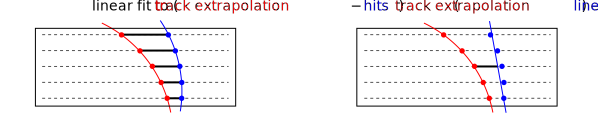
\includegraphics[width=\linewidth]{segment_residuals.pdf}

\vfill \begin{itemize}
\item Only matters when the muon is expected to curve significantly inside the chamber, e.g.\ ME1/1 and ME1/2
\begin{itemize}
\item probably negligible the DTs
\end{itemize}
\end{itemize}
\end{frame}

\begin{frame}
\frametitle{Residuals weights}

\vspace{-0.5 cm}
\begin{itemize}\setlength{\itemsep}{0.25 cm}
\item ``Bad'' segments distort residuals distribution, so weight segment residuals by their $(\chi^2/N_{\mbox{\scriptsize dof}})^{-1}$ (good fits get the most weight)
\item Normalized with $\langle (\chi^2/N_{\mbox{\scriptsize dof}})^{-1} \rangle = 1.0$, so that errors are meaningful
\item The usual dangers with weights are:
\begin{itemize}\setlength{\itemsep}{0.1 cm}
\item parameterized hit uncertainties {\it might} be unrepresentative
\item unphysically low-weight events can bias a distribution \\ (they
  appear as spikes in a histogram)
\end{itemize}
\item Not an issue with these weights because:
\begin{itemize}\setlength{\itemsep}{0.1 cm}
\item consistency with a line is a geometric \\ attribute, not very sensitive to the \\ precise hit uncertainties
\item we exclude the lowest 1\% of weights
\end{itemize}
\item {\it Necessary} for good fits in wheel $\pm$2, station 1 $\Delta \frac{dy}{dz}$ (above)
\end{itemize}

\vspace{-4 cm}
\hfill \includegraphics[width=0.33\linewidth]{wheel2_station1_dydz.png}
\end{frame}

\begin{frame}
\frametitle{Treatment of residuals (1/4)}

\begin{itemize}\setlength{\itemsep}{0.2 cm}
\item Residuals are influenced by misalignment geometry and propagation/instrumental effects:
\begin{itemize}\setlength{\itemsep}{0.2 cm}
\item misalignments distort residuals according to an exact \mbox{6$\times$4 matrix\hspace{-1 cm}}
\item some propagation errors are Gaussian (statistical error,
  multiple scattering, etc.) and some power-law (single-scattering)
\item propagation correlates $\Delta x$ with $\Delta \frac{dx}{dz}$ and $\Delta y$ with $\Delta \frac{dy}{dz}$

\mbox{ } \hfill \includegraphics[width=0.8\linewidth]{propagation_correlation.pdf} \hfill \hfill \mbox{ }

\item sources of systematic error to be quantified or controlled: tracker misalignment, imperfect $\vec{B}(\vec{x})$ and material maps, internal DT misalignment
\end{itemize}

\item All of the above are convoluted together in an 9 dimensional space:

\mbox{($\Delta x$, $\Delta \frac{dx}{dz}$, $\Delta y$, $\Delta \frac{dy}{dz}$, $x$ position, $\frac{dx}{dz}$ angle, $y$ position, $\frac{dy}{dz}$ angle, $q/p_T$)\hspace{-1 cm}}
\end{itemize}
\end{frame}

\begin{frame}
\frametitle{What HIP does (2/4)}

\begin{itemize}\setlength{\itemsep}{0.1 cm}
\item Incorporate misalignment, Gaussian and Lorentzian propagation
  effects, with $\Delta x$-$\Delta \frac{dx}{dz}$ correlations, into a \textcolor{blue}{single ansatz}
\begin{itemize}
\item 6 alignment parameters, $\sigma$ and $\Gamma$ for each of the 4 residuals, 2~correlation parameters = 16 parameters \mbox{for each DT$_{\mbox{\scriptsize station 1--3}}$\hspace{-1 cm}}
\item 3-way convolution: 

\vspace{-0.35 cm}
\[ \mbox{residuals} = [\mbox{Gaussian} \otimes \mbox{Lorentzian}](\mbox{misalignment}) \]
\end{itemize}

\item \textcolor{blue}{Fit all chamber variables simultaneously} {\scriptsize (unbinned log-likelihood)}
\begin{itemize}
\item include all the physical tails {\scriptsize (cut unphysical $|\Delta x_i|\mbox{, }|\Delta y_i| < 1000$~cm)}
\item seed fit with truncated means and standard deviations \mbox{for stability\hspace{-1 cm}}
\item project the fit results on all axes to make sure it's working
\end{itemize}

\item Usually separate two $q/p_T$ bins to account for the $\vec{B}(\vec{x})$ and $dE/dx(\vec{x})$ instrumental effects {\scriptsize (but turned off for this alignment)}

\item Tracker and DT internal alignment are external inputs, assumed to be correct and worth investigating as systematics studies
\begin{itemize}
\item quantified misalignment scenarios test sensitivity in \mbox{MC \scriptsize (e.g.\ CSA08)\hspace{-1 cm}}
\item non-pointing cosmic rays reveal global distortions {\scriptsize (e.g.~TEC)}
\item $p_T$ dependence provides some information {\scriptsize (e.g.~tracker curl study)}
\end{itemize}
\end{itemize}
\end{frame}

\begin{frame}
\frametitle{What MillePede does (3/4)}

\begin{columns}
\column{0.5\linewidth}
\begin{enumerate}
\item Fit peaks of residuals distributions to Lorentzian \mbox{(or Gaussian)} to identify a [peak $-$ $\sigma$, peak $+$ $\sigma$] window
\item Compute the residuals $\to$ alignment corrections inversion for all hits in the window
\end{enumerate}

\column{0.5\linewidth}
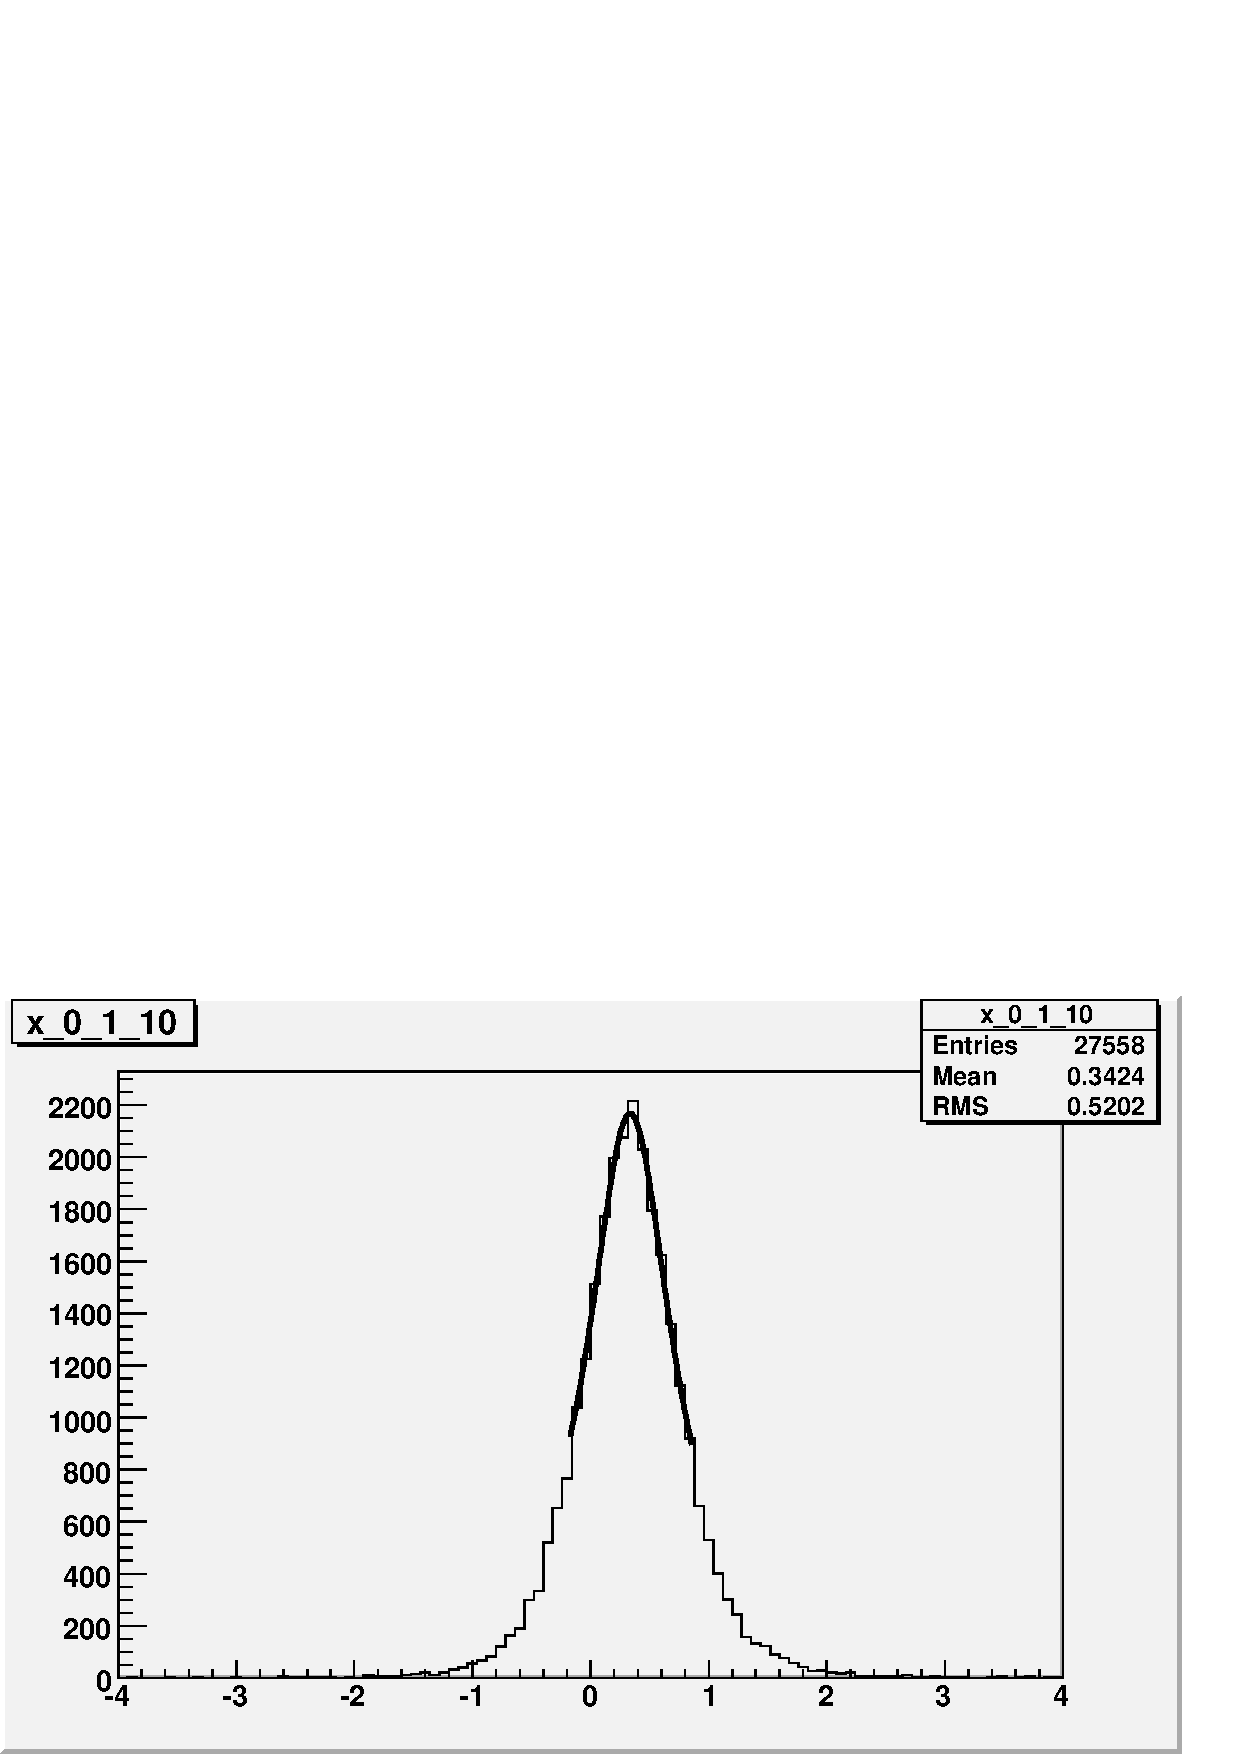
\includegraphics[width=0.9\linewidth]{canvas_x_0_1_10.pdf}
\end{columns}

\vspace{0.2 cm}
\mbox{\hspace{-0.34 cm}\begin{minipage}{\linewidth}
\begin{itemize}\setlength{\itemsep}{-0.01 cm}
\item \textcolor{blue}{All alignment parameters are fitted simultaneously, but residuals tails from propagation effects are explicitly cut out}
\begin{itemize}
\item this is a matrix-mean: in a 1-DOF case (e.g.\ aligning $\delta_x$ only), it is equivalent to a computation of the mean within the selected window
\item trade-off: loose cut lets in non-Gaussian tails, tight cut introduces a dependence on its value
\end{itemize}

\item Control $\vec{B}(\vec{x})$ and $dE/dx(\vec{x})$ instrumental effects with a linear $q/p_T$ fit {\scriptsize (but turned off for this alignment)}

\item Same systematics issues as HIP

\end{itemize}\end{minipage}}
\end{frame}

\begin{frame}
\frametitle{My commentary (4/4)}

\begin{itemize}\scriptsize
\item The mean of a distribution with such a tight cut (deep in the
  bulk of the distribution) would depend on the placement of the cut boundary
\item {\it However,} the perfect symmetry of [peak $-$ $\sigma$, peak
  $+$ $\sigma$] should balance the residuals on each side of the peak,
  as long as the pre-fit is a good fit $\surd$
\item {\it However,} the matrix inversion depends on trends in the
  residuals distributions, which may not be as well balanced
\begin{itemize}\setlength{\itemsep}{0.1 cm}\scriptsize
\item for example, a term contributing to $\delta_{\phi_z}$ alignment
  is the slope of \\ $\Delta x$ residuals versus $y$ position (there are many other terms like this)
\item the slope can be distorted by a tight cut:

\begin{center}
\includegraphics[width=0.8\linewidth]{residuals_with_a_cut.pdf}
\end{center}
\end{itemize}
\item The example I drew has misalignment $\sim$ residuals $\sigma$,
  which would be about 4~mrad for $\phi_z$

\item Monte Carlo can verify whether the MillePede alignment is sensitive
  to these sorts of effects
\end{itemize}
\end{frame}

\begin{frame}
\frametitle{Error in the MP matrix? (1/2)}
\scriptsize

\begin{itemize}
\item HIP alignment matrix, presented last month with a suite of MC tests

(including turning off measurement error to observe pure geometric effects)

\vspace{-0.5 cm}
\[ \renewcommand{\arraystretch}{1.5}
\left(\begin{array}{c}
{\Delta x} \\
{\Delta y} \\
{\Delta \frac{dx}{dz}} \\
{\Delta \frac{dy}{dz}} \\
\end{array}\right)
=
\left(\begin{array}{c c c c c c}
-1 & \textcolor{white}{-}0 & \frac{dx}{dz} & y \frac{dx}{dz} & -x \frac{dx}{dz} & \textcolor{white}{-}y \\
\textcolor{white}{-}0 & -1 & \frac{dy}{dz} & y \frac{dy}{dz} & -x \frac{dy}{dz} & -x \\
\textcolor{white}{-}0 & \textcolor{white}{-}0 & \textcolor{blue}{0} & \textcolor{blue}{\frac{dx}{dz} \frac{dy}{dz}} & \textcolor{blue}{-1 - \left(\frac{dx}{dz}\right)^2} & \textcolor{white}{-}\frac{dy}{dz} \\
\textcolor{white}{-}0 & \textcolor{white}{-}0 & \textcolor{blue}{0} & \textcolor{blue}{1 + \left(\frac{dy}{dz}\right)^2} & \textcolor{blue}{-\frac{dx}{dz}\frac{dy}{dz}} & -\frac{dx}{dz}
\end{array}\right)
\renewcommand{\arraystretch}{1.05}
\left(\begin{array}{c}
\delta_x \\
\delta_y \\
\delta_z \\
\delta_{\phi_x} \\
\delta_{\phi_y} \\
\delta_{\phi_z}
\end{array}\right)
\]

\item MP alignment matrix in SegmentAlignmentDerivatives4D.cc

\vspace{-0.25 cm}
\[ \renewcommand{\arraystretch}{1.5}
\left(\begin{array}{c}
{\Delta x} \\
{\Delta y} \\
{\Delta \frac{dx}{dz}} \\
{\Delta \frac{dy}{dz}} \\
\end{array}\right)
=
\left(\begin{array}{c c c c c c}
-1 & \textcolor{white}{-}0 & \frac{dx}{dz} & y \frac{dx}{dz} & -x \frac{dx}{dz} & \textcolor{white}{-}y \\
\textcolor{white}{-}0 & -1 & \frac{dy}{dz} & y \frac{dy}{dz} & -x \frac{dy}{dz} & -x \\
\textcolor{white}{-}0 & \textcolor{white}{-}0 & \textcolor{blue}{\frac{dx}{dz}} & \textcolor{blue}{0} & \textcolor{blue}{-1} & \textcolor{white}{-}\frac{dy}{dz} \\
\textcolor{white}{-}0 & \textcolor{white}{-}0 & \textcolor{blue}{\frac{dy}{dz}} & \textcolor{blue}{1} & \textcolor{white}{-}\textcolor{blue}{0} & -\frac{dx}{dz}
\end{array}\right)
\renewcommand{\arraystretch}{1.05}
\left(\begin{array}{c}
\delta_x \\
\delta_y \\
\delta_z \\
\delta_{\phi_x} \\
\delta_{\phi_y} \\
\delta_{\phi_z}
\end{array}\right)
\]

\item First column of differences \textcolor{blue}{(blue)} say that $\delta_z$ misalignment causes angle residuals (e.g.~$\Delta \frac{dx}{dz} = \delta_z \, \frac{dx}{dz}$)

\item Second two columns are an approximation that $\frac{dx}{dz}$ and $\frac{dy}{dz}$ are small

\mbox{($\left|\frac{dx}{dz}\right|$ reaches 0.25 in every chamber, $\left|\frac{dy}{dz}\right|$ reaches 0.7 in wheel $\pm$1 and 0.9 in $\pm$2)\hspace{-1 cm}}
\end{itemize}
\end{frame}

\begin{frame}
\frametitle{Error in the MP matrix? (2/2)}
\begin{itemize}
\item Biggest discrepancy between HIP and MP is in local $\delta_z$, and the biggest difference between the matrices contributes to $\delta_z$
\item $\delta_z$ translations do not change segment angles: \hfill \mbox{\vspace{-0.5 cm}\begin{minipage}{2.5 cm}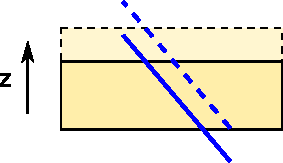
\includegraphics[width=\linewidth]{matrix_error_z.pdf}\end{minipage}}
\item A Monte Carlo test would catch this immediately
\end{itemize}

\vspace{0.5 cm}
\hspace{-0.83 cm} \textcolor{darkblue}{\Large Cosmic ray Monte Carlo}

\begin{itemize}
\item Summer08 tracker-pointing AlCaReco skims available
\item Everything is the same as in CRAFT data except:
\begin{itemize}\setlength{\itemsep}{0.1 cm}
\item ideal tracker alignment, magnetic field, and \mbox{DT internal alignment\hspace{-1 cm}}
\item about 4 times the sample size
\end{itemize}

\item All HIP/MP implementation differences should be modeled by MC
\begin{itemize}
\item if not, we can add realistic tracker, field, and DTs to diagnose
\end{itemize}
\end{itemize}
\end{frame}

\begin{frame}
\frametitle{HIP accuracy in MC}

\begin{itemize}
\item Same convergence as in data (2 iterations necessary, 3 taken)
\item 200~$\mu$m in $r\phi$ (with about 4 times as many tracks)
\item More accurate in $y$ and $z$ than collisions MC test because of \mbox{high $p_T$\hspace{-1 cm}}

\scriptsize (Local $z$ is degenerate with $q$-antisymmetric effects like $\vec{B}$ and $dE/dx$)
\end{itemize}

\vfill
\includegraphics[height=\linewidth, angle=90]{hip_MC.pdf}
\end{frame}

\begin{frame}
\frametitle{HIP Normalized distributions}

\begin{itemize}
\item Statistical uncertainties are 3--4$\times$ smaller than accuracy
\end{itemize}

\vfill
\includegraphics[height=\linewidth, angle=90]{hip_MCnorm.pdf}
\end{frame}

\begin{frame}
\frametitle{HIP uncertainties}

\begin{itemize}
\item Define $\mbox{systematic error} = \sqrt{\mbox{(absolute error)}^2 - \mbox{(statistical)}^2}$
\begin{itemize}\setlength{\itemsep}{0.1 cm}
\item this ``systematic'' doesn't include tracker misalignments, imperfect $\vec{B}$ map, DT internal misalignments
\item we expect statistical to scale with $\sqrt{N}$, but not systematic
\end{itemize}
\end{itemize}

\vfill
\includegraphics[height=\linewidth, angle=90]{hip_MCuncertainties.pdf}
\end{frame}

\begin{frame}
\frametitle{Proposed constants}
\begin{itemize}
\item Pablo and I did not get to talk about proposing constants, and I
  have not seen the MillePede Monte Carlo results
\item What I know is:
\begin{itemize}\setlength{\itemsep}{0.1 cm}
\item the constants from the two implementations differ
\item the $\pm$1~$\sigma$ cut in residuals can distort results derived from slopes
\item the error matrix in SegmentAlignmentDerivatives4D.cc will cause
  errors in $z$ (and propagate to $y$ for wheels~$\pm$1)
\item the HIP procedure is well-behaved in cosmic ray Monte Carlo
\item if there are global distortions in the tracker, it would not affect HIP and MP differently
\end{itemize}
\item Therefore, I will propose the HIP results, show the validation, and list all of the known mysteries

{\scriptsize \it (All cuts and parameters for this alignment were listed on pages 3--4)}
\end{itemize}
\end{frame}

\begin{frame}
\frametitle{DB comparisons (\only<1>{1}\only<2>{2}/5)}
\framesubtitle{CRAFT\_ALL\_V4 $-$ proposed constants}

\begin{itemize}
\item CRAFT\_ALL\_V4 is before global alignment
\item We have seen these large absolute $\delta_x$ corrections before:
  they preserve local alignment within sectors (like moving fingers)
\end{itemize}

\only<1>{\includegraphics[height=\linewidth, angle=90]{hip_difference_v4.pdf}}\only<2>{\includegraphics[height=\linewidth, angle=90]{hip_difference2_v4.pdf}}

\tiny \textcolor{red}{This plot now uses the latest tracker!}
\end{frame}

\begin{frame}
\frametitle{DB comparisons (\only<1>{3}\only<2>{4}/5)}
\framesubtitle{CRAFT\_ALL\_V11 $-$ proposed constants}

\begin{itemize}\scriptsize
\item CRAFT\_ALL\_V11 is the first global alignment
\item The wheel rotation is a known effect, related solely to difference in momentum cuts (and also preserves local alignments):
\begin{itemize}
\item old: $20 < p_T < 100$~GeV, \hfill new: $100 < p_T < 200$~GeV \hfill \mbox{ }
\end{itemize}
\end{itemize}

\only<1>{\includegraphics[height=0.95\linewidth, angle=90]{hip_difference_v11all.pdf}}\only<2>{\includegraphics[height=0.95\linewidth, angle=90]{hip_difference2_v11all.pdf}}

\tiny \textcolor{red}{This plot now uses the latest tracker!}
\end{frame}

\begin{frame}
\frametitle{Rotation with high $p_T$ (5/5)}

\begin{itemize}
\item These plots show the difference between low $p_T$ and high $p_T$ (everything else is the same; this is a systematics study)
\begin{itemize}
\item global coordinates: $\Delta \phi$ (top) is rotation around beamline, \\ $r\phi$ (bottom) is the same orientation for all chambers
\end{itemize}
\item 0.35 mrad rotation, 0.04 mrad/m twist, and 3.2 mm spread
\end{itemize}

\includegraphics[height=\linewidth, angle=90]{data_effect_of_100GeVcut3.pdf}
\end{frame}

\begin{frame}
\frametitle{Studies of $p_T$ effect (1/2)}
\framesubtitle{Alignments from low and high $p_T$ differ: how do we know which is right?}

\begin{itemize}
\item Ratio of tracker $p_T$ and globalMuon $p_T$ vs.\ momentum in CRAFT
\item Study repeated with low and high $p_T$ alignments {\scriptsize (from prev page)}
\item Alignment made with high $p_T$ (solid \textcolor{red}{red} and black) yields more correct ratios (1.0) at all momenta
\end{itemize}

\vfill\includegraphics[width=\linewidth]{cosmicsplitting_nhan.png}
\end{frame}

\begin{frame}
\frametitle{Studies of $p_T$ effect (2/2)}
\framesubtitle{Alignments from low and high $p_T$ differ: how do we know which is right?}
\scriptsize

\begin{itemize}
\item Cosmic track splitting: difference between top and bottom half of cosmic ray
\item Tracks with station~1 muon hits (\textcolor{green}{TPFMS} and TMR) yield better resolution than \textcolor{red}{tracker only (TO)} for the first time!
\begin{itemize}\scriptsize
\item this was not the case for the low-$p_T$ alignment, or any previous alignments
\end{itemize}
\item Highest-$p_T$ bin in this study \mbox{is statistically independent of 100--200~GeV alignment\hspace{-1 cm}}
\end{itemize}

\hfill \scriptsize \textcolor{darkblue}{J.~Tucker}

\vspace{-\baselineskip}
\includegraphics[width=0.87\linewidth]{cosmicsplitting_jordan.png}
\end{frame}

\begin{frame}
\frametitle{$p_T$ effect in raw residuals}

\includegraphics[width=0.45\linewidth]{resid_vs_pt.pdf} \hfill \includegraphics[width=0.45\linewidth]{resid_vs_qoverpt.pdf}

\begin{itemize}
\item Single chamber {\scriptsize (wheel~0, station~1, sector~10, bottom of barrel)}
\item $\mu^+$/$\mu^-$ splitting at low $p_T$ is due to $\vec{B}(\vec{x})$ and $dE/dx$ errors
\item Charge-independent variation with $p_T$ is not
\item Not the same shape in all chambers
\end{itemize}
\end{frame}

\begin{frame}
\frametitle{$\frac{dx}{dz}$ (sawtooth variable) and $p_T$}

\begin{columns}
\column{0.35\linewidth}
\vspace{0.25 cm}
\includegraphics[width=\linewidth]{cosmics_are_nasty.pdf}

\column{0.65\linewidth}
\begin{itemize}
\item Still looking at only one chamber, note that $\frac{dx}{dz}$ and $p_T$ are related
\item Expected because low-$p_T$ muons are more vertically collimated by the Earth
\item \textcolor{darkblue}{Unique to cosmic rays: in $\phi$-symmetric collisions, $p_T$ and $\frac{dx}{dz}$ will be independent}
\end{itemize}
\end{columns}

\vspace{-0.25 cm}
\begin{columns}
\column{0.2\linewidth}
\begin{itemize}
\item Low-$p_T$ band is sloped because of $\vec{B}$
\end{itemize}

\column{0.8\linewidth}
\includegraphics[height=\linewidth, angle=90]{sawtooth_and_qoverpt2.pdf}
\end{columns}
\end{frame}

\begin{frame}
\frametitle{Dependence on both $p_T$ and $\frac{dx}{dz}$}

\begin{itemize}
\item Residuals (greyscale, mm) are a function of both $p_T$ and $\frac{dx}{dz}$
\begin{itemize}\setlength{\itemsep}{0.1 cm}
\item sawtooth effect is vertical trend from dark to light
\item $p_T$ effect is horizontal darkening in center
\end{itemize}
\item Sawtooth and $p_T$ effect may be related
\end{itemize}
\includegraphics[height=\linewidth, angle=90]{sawtooth_qoverpt_complicated2.pdf}
\end{frame}

\begin{frame}
\frametitle{Verification with segments (\only<1>{1}\only<2>{2}/2)}

\only<1>{\includegraphics[width=0.33\linewidth]{alicia_rphiB.png}
\includegraphics[width=0.33\linewidth]{alicia_rphiC.png}
\includegraphics[width=0.33\linewidth]{alicia_rphiD.png}}
\only<2>{\includegraphics[width=0.33\linewidth]{alicia_phiyB.png}
\includegraphics[width=0.33\linewidth]{alicia_phiyC.png}
\includegraphics[width=0.33\linewidth]{alicia_phiyD.png}}

\begin{columns}
\column{0.5\linewidth}
\only<1>{\includegraphics[height=\linewidth, angle=90]{RPhires_YB0YB1YBm1_HIPiter03_InOut_38T-1.pdf}}
\only<2>{\includegraphics[height=\linewidth, angle=90]{Phires_YB0YB1YBm1_HIPiter03_InOut_38T-1.pdf}}
\column{0.5\linewidth}
\only<1>{\begin{itemize}
\item Segment-matching among stations 1--3 yields $\sim$800~$\mu$m
\item Station 4 RMS is dominated by a few outliers, mostly in sector~4
\end{itemize}}
\only<2>{\begin{itemize}
\item Segment angle-matching is $\sim$0.7~mrad
\end{itemize}}

\vspace{0.5 cm}
\end{columns}

\vspace{-\baselineskip}
\hfill \textcolor{darkblue}{A.~Calderon}
\end{frame}

\begin{frame}
\frametitle{Station 4 outliers}

Segment-extrapolation plots:

\vfill
\mbox{\hspace{-0.75 cm}\includegraphics[width=1.15\linewidth]{alicia_outliers.png}}

\begin{itemize}
\item Station 4, sector 4 is always an outlier
\begin{itemize}
\item it has an apparent internal misalignment (next slide)
\item detailed fit results on next slide
\end{itemize}

\item Wheel $+$1, station 4, sector 9 became an outlier at high $p_T$
\begin{itemize}
\item low statistics $+$ non-uniform coverage?
\item detailed fit results on in two slides
\end{itemize}

\end{itemize}
\end{frame}

\begin{frame}
\frametitle{Wheel $+$1, station 4, sector 4}

\includegraphics[height=0.7\linewidth, angle=90]{bell_MBwhDst4sec04.pdf}\includegraphics[width=0.3\linewidth]{station4_sector4.png}

\vspace{0.5 cm}
\includegraphics[height=\linewidth, angle=90]{poly_MBwhDst4sec04.pdf}

\vspace{-1 cm}
\end{frame}

\begin{frame}
\frametitle{Reminder from Apr 27}

\begin{columns}
\column{0.7\linewidth}
\begin{itemize}
\item This is what wheel~0, station~4, sector~4 looked like with high statistics (low-$p_T$ alignment)
\item It {\it really} looks like a misalignment between the two halves of the chambers in this sector
\end{itemize}

\column{0.3\linewidth}
\includegraphics[width=\linewidth]{station4_sector4.png}
\end{columns}

\vspace{0.5 cm}
\includegraphics[height=\linewidth, angle=90]{datafit_st4sec_04_13.pdf}

\vspace{-1 cm}
\end{frame}

\begin{frame}
\frametitle{Wheel $+$1, station 4, sector 9}

\includegraphics[height=\linewidth, angle=90]{bell_MBwhDst4sec09.pdf}

\vspace{0.5 cm}
\includegraphics[height=\linewidth, angle=90]{poly_MBwhDst4sec09.pdf}

\vspace{-1 cm}
\end{frame}

\begin{frame}
\frametitle{Sawtooth effect (\only<1>{1}\only<2>{2}\only<3>{3}/3)}

\vspace{0.25 cm}
\begin{itemize}\scriptsize
\item Slope in $\Delta \frac{dx}{dz}$ versus $\frac{dx}{dz}$ which
  feeds into other diagnostic plots due to the correlation between
  $\Delta x$ and $\Delta \frac{dx}{dz}$ and the correlation between
  $x$ and $\frac{dx}{dz}$
\item Not a rigid body misalignment of the whole chamber, but can be related to internal layer $\delta_x$ corrections
\item<2-3> Largest in wheel $-$1, with a sinusoidal structure
\end{itemize}

\vfill
\only<1>{\includegraphics[height=\linewidth, angle=90]{sawtooth_bysector_highp_newinternal_zalign_fits.pdf}}
\only<2>{\includegraphics[height=\linewidth, angle=90]{sawtooth_bysector_highp_newinternal_zalign_fits2.pdf}}
\only<3>{\includegraphics[height=\linewidth, angle=90]{sawtooth_bysector_highp_newinternal_zalign_fits3.pdf}}
\end{frame}

\begin{frame}
\frametitle{Summary of HIP alignment}
\begin{itemize}
\item Simultaneous solution of alignment and propagation effects \\ {\scriptsize (which are not easily separable due to convolution)}
\item Method verified in cosmics Monte Carlo with high \mbox{accuracy (200~$\mu$m),\hspace{-1 cm}} {\scriptsize including geometry-only test of residuals $\leftrightarrow$ alignment corrections matrix}
\item Alignment in data verified by:
\begin{enumerate}\scriptsize
\item ratio of tracker $p_T$ to globalmuon $p_T$: discovered source of rotation
\item cosmic ray track splitting: first alignment which improves upon tracker
\item segment extrapolation: 800~$\mu$m in stations 1--3
\end{enumerate}

{\scriptsize \textcolor{darkblue}{(1)} Nhan Tran, \textcolor{darkblue}{(2)} Jordan Tucker and Nhan Tran, \textcolor{darkblue}{(3)} Alicia Calderon}

\item What we don't understand:
\begin{itemize}
\item origin of charge-independent variation of residuals with $p_T$ (though we know that high $p_T$ is more correct)
\item sawtooth effect (non rigid-body variation of residuals with $\frac{dx}{dz}$)
\end{itemize}

\item These conditions are external to the alignment algorithm and should affect MillePede equally

\item \scriptsize Note that alignment will need to be repeated, with exactly the same parameters and the new tracker alignment and APEs when they become available
\end{itemize}
\label{numpages}
\end{frame}

%% \begin{frame}
%% \frametitle{Outline}
%% \begin{itemize}\setlength{\itemsep}{0.75 cm}
%% \item 
%% \end{itemize}
%% %% \hspace{-0.83 cm} \textcolor{darkblue}{\Large Outline2}
%% \end{frame}

%% \section*{First section}
%% \begin{frame}
%% \begin{center}
%% \Huge \textcolor{blue}{First section}
%% \end{center}
%% \end{frame}

\begin{frame}
\frametitle{Timeline of updates}
\framesubtitle{All dates correspond to talks where I presented the updates}
\scriptsize

\vfill
\mbox{\hspace{-0.5 cm}\renewcommand{\arraystretch}{1.1}\begin{tabular}{c p{0.75\linewidth}}
Nov~11,~2008 & First CRAFT globalMuon alignment attempt: combining residuals from all chambers in each wheel, observed rotation $+$ twist \\
 & Control $\vec{B}$ with $q/p_T$ extrapolation \\
Nov~24 & Used muon residuals to x-ray tracker, observed TEC misalignment \\
Jan~21,~2009 & Split residuals by chamber, rotation $+$ twist disappeared (low $p_T$) \\
 & Gaussian $\otimes$ Lorentzian convolution to model residuals tails \\
 & Detailed residuals maps show discontinuities at chamber boundaries: only evidence of global structure in tracks from TEC \\
 & Excluded tracks from TID/TEC, control $\vec{B}$ with two-bin method \\
Jan~29 & Signed-off $x$, $y$, $\phi_z$ chamber-by-chamber constants from 1-D fits with tails, only about half the chambers (now known as CRAFT\_ALL\_V11) \\
Jan~28 and Feb~5 & First study of sawtooth: not a rigid-body misalignment ($z$ or $\phi_y$) \\
Feb~20 & Detailed MC scenario based on CRAFT\_ALL\_V11 alignment \\
Mar~31, Apr~2, Apr~14 & Updates in expanding 1-D fits into a combined 6-DOF fit \\
 & Wrote 40-page track-based alignment note \\
Apr~27 & Presented complete 6-DOF alignment with systematics studies and MC study (but low $p_T$), not accepted for sign-off \\
May~11 & Discovered $q$-symmetric $p_T$ dependence and origin of old rotation $+$ twist, followed-up with resolution studies in POG \\
May~18 & Discovered global structure in sawtooth distribution \\
May~25 & Proposing a high-$p_T$ HIP alignment for sign-off \\
\end{tabular}}
\end{frame}

\begin{frame}
\frametitle{Changes since last alignment}
\scriptsize

\vspace{0.25 cm}
\renewcommand{\arraystretch}{1.35}\begin{tabular}{p{0.45\linewidth} p{0.53\linewidth}}
CRAFT\_ALL\_V11 global alignment & This HIP alignment \\\hline
Tight criteria for accepting an aligned chamber; only half of DTs passed & Loose criteria (5 hits and a successful fit), only 3 fail within selected region: wheels $-$1, 0, $+$1, all sectors except 1 and 7 \\
$x$, $y$, $\phi_z$ only from independent 1-D fits & All 6 DOF from a combined fit, though station~4 is only $x$, $\phi_y$, $\phi_z$ \\
Combining hits into segment-residuals only for their statistical properties & Also using angular information for tighter control of DOF \\
$20 < p_T < 100$~GeV & $100 < p_T < 200$~GeV \\
Control $\vec{B}$ with two-bin method & Temporarily turn off $\vec{B}$ control (not needed at this high momentum) \\
No residuals weights & Weight residuals by $(\chi^2/N_{\mbox{\scriptsize dof}})^{-1}$ \\
2 iterations & 3 iterations (third not needed) \\
Require 10 tracker hits, no TID/TEC & Require 15 tracker hits (for synchronization with MillePede), no TID/TEC \\
CMSSW\_2\_2\_7, tracker alignment, APEs, and $\vec{B}$ map of that time & CMSSW\_2\_2\_11, new tracker alignment, APEs, $\vec{B}$ map \\
Internal DT alignment from CRAFT\_ALL\_V4 & New internal DT alignment (with tracks-survey agreement) \\
Data source: first CRAFT reprocessing & Latest CRAFT tracker-pointing reprocessing \\
\end{tabular}
\end{frame}

\begin{frame}
\frametitle{Tracker curl hypothesis}
\framesubtitle{$p_T$-dependent rotation could be curl in tracker, if large enough}
\includegraphics[width=\linewidth]{curl_explanation.pdf}
\end{frame}

\begin{frame}
\frametitle{Tracker curl constraints}

\includegraphics[width=0.55\linewidth]{tracks_are_sensitive_to_curl.png} \hfill \includegraphics[width=0.35\linewidth]{curl_is_not_86microns.png}

\begin{itemize}
\item Studies performed in CRAFT data \hfill \textcolor{darkblue}{\scriptsize Zijin Guo, Roberto Castello}
\item \textcolor{darkblue}{Left:} tracker tracks are sensitive to 300~$\mu$rad curl (\textcolor{blue}{blue:\ adding curl worsens $\chi^2$} and \textcolor{red}{red:\ re-aligning restores it})
\item \textcolor{darkblue}{Right:} also restores wafer positions within 150~$\mu$rad \mbox{except TEC\hspace{-1 cm}}
\begin{itemize}
\item TEC not used in muon alignment; not relevant here
\item restored chamber positions randomly distributed around zero: \textcolor{darkblue}{no {\it systematic} trend on the scale of 86~$\mu$rad}
\end{itemize}
\end{itemize}
\end{frame}

\begin{frame}
\frametitle{All the numbers}
\framesubtitle{Relative to ideal in mm and mrad}
\tiny
\vspace{0.1 cm}
\mbox{\hspace{-0.75 cm}\begin{tabular}{c c c c}
wheel & CRAFT\_ALL\_V4 (before global alignment) & CRAFT\_ALL\_V11 & This HIP alignment \\
station & $x$, $y$, $z$, $\phi_x$, $\phi_y$, $\phi_z$ & $x$, $y$, $\phi_z$ & $x$, $y$, $z$, $\phi_x$, $\phi_y$, $\phi_z$ \\
sector & & {\it (unaligned in italics)} & {\it (unaligned in italics)} \\\hline
-1, 1, 2 &  -5.28,   -1.02,   -3.54,   1.10,   -1.65,   -0.50,  &  {\it (0.19),}   -1.27,   {\it (0.44),}  &  0.36,   1.02,   -4.09,   3.51,   1.06,   0.89,  \\
-1, 1, 3 &  -3.14,   -0.74,   2.09,   0.77,   -1.17,   -0.00,  &  1.33,   -0.01,   0.48,  &  0.62,   2.67,   3.00,   0.60,   -2.35,   0.24,  \\
-1, 1, 4 &  -0.32,   0.28,   4.89,   1.98,   0.93,   -0.29,  &  1.54,   1.94,   -0.32,  &  1.70,   3.16,   6.14,   2.03,   -0.04,   -0.18,  \\
-1, 1, 5 &  4.51,   -0.38,   1.78,   0.29,   1.63,   -0.35,  &  3.82,   {\it (1.78),}   -0.88,  &  5.70,   1.36,   7.08,   -0.96,   2.74,   -1.14,  \\
-1, 1, 6 &  0.64,   -1.24,   -2.95,   0.50,   1.83,   -0.80,  &  {\it (-0.26),}   -1.24,   {\it (-0.80),}  &  4.10,   0.64,   -0.58,   -0.82,   4.51,   -0.00,  \\
-1, 1, 8 &  -1.90,   -0.04,   -3.37,   -0.95,   -2.13,   0.18,  &  0.38,   1.39,   -1.38,  &  1.79,   3.19,   -1.58,   0.38,   -1.13,   -1.16,  \\
-1, 1, 9 &  -2.24,   -1.16,   1.84,   -0.58,   -1.78,   0.44,  &  0.27,   0.18,   -1.05,  &  2.15,   1.01,   5.32,   -0.15,   -2.31,   -0.93,  \\
-1, 1, 10 &  -0.08,   0.36,   5.31,   1.91,   0.69,   -0.02,  &  2.29,   0.24,   0.13,  &  4.94,   -0.38,   7.86,   1.09,   0.11,   0.29,  \\
-1, 1, 11 &  3.60,   -0.46,   0.96,   1.48,   2.49,   -0.11,  &  7.45,   -2.79,   0.20,  &  9.82,   -3.91,   7.10,   -1.09,   2.06,   0.30,  \\
-1, 1, 12 &  2.63,   0.45,   -3.90,   1.44,   2.54,   0.02,  &  6.57,   0.56,   0.92,  &  {\it (2.63,}   {\it 0.45,}   {\it -3.90,}   {\it 1.44,}   {\it 2.54,}   {\it 0.02),}  \\
-1, 2, 2 &  -5.29,   2.12,   -4.56,   0.22,   -1.78,   0.27,  &  1.11,   0.91,   1.19,  &  1.52,   2.40,   -4.81,   -1.05,   -4.05,   1.02,  \\
-1, 2, 3 &  -4.37,   -0.74,   0.77,   -0.49,   -1.67,   -0.67,  &  {\it (1.97),}   -0.81,   {\it (0.19),}  &  0.80,   4.06,   -0.23,   -3.41,   -2.30,   0.06,  \\
-1, 2, 4 &  -1.63,   -0.26,   3.75,   -0.08,   -1.36,   -0.15,  &  1.15,   1.03,   -0.16,  &  1.67,   2.75,   5.08,   -1.21,   -1.95,   -0.11,  \\
-1, 2, 5 &  4.03,   -2.28,   1.60,   0.06,   0.61,   -0.31,  &  {\it (1.81),}   {\it (-0.55),}   {\it (0.37),}  &  4.66,   -2.73,   12.06,   -3.06,   2.15,   0.22,  \\
-1, 2, 6 &  3.06,   -0.73,   -3.87,   -0.53,   1.10,   0.29,  &  1.40,   -4.08,   -1.17,  &  4.48,   -3.19,   1.95,   -3.13,   3.39,   -0.25,  \\
-1, 2, 8 &  -0.83,   -1.06,   -4.94,   -0.98,   -2.36,   -0.65,  &  {\it (0.97),}   -1.06,   {\it (-0.65),}  &  {\it (-0.83,}   {\it -1.06,}   {\it -4.94,}   {\it -0.98,}   {\it -2.36,}   {\it -0.65),}  \\
-1, 2, 9 &  -1.99,   -1.28,   0.81,   -1.20,   -1.92,   0.25,  &  {\it (-1.99),}   {\it (-1.28),}   {\it (0.25),}  &  2.45,   1.49,   5.03,   -2.11,   -3.18,   0.26,  \\
-1, 2, 10 &  -0.15,   -0.83,   4.97,   -0.10,   0.10,   0.26,  &  1.51,   {\it (-0.83),}   0.26,  &  5.86,   -1.09,   7.61,   -0.54,   -0.54,   0.47,  \\
-1, 2, 11 &  2.40,   -0.35,   1.30,   -0.67,   1.67,   -0.13,  &  6.55,   -4.02,   0.68,  &  11.30,   -3.82,   5.98,   -2.59,   1.14,   -0.62,  \\
-1, 2, 12 &  0.90,   -0.44,   -4.58,   1.13,   1.79,   -0.77,  &  5.17,   -1.26,   0.51,  &  10.54,   -2.42,   3.88,   -2.78,   0.62,   0.87,  \\
-1, 3, 2 &  -4.15,   -2.75,   -4.37,   -0.17,   -1.19,   -0.26,  &  3.60,   0.68,   1.23,  &  3.18,   1.50,   -2.31,   -0.70,   -3.07,   0.76,  \\
-1, 3, 3 &  -3.17,   -1.33,   1.20,   0.36,   -1.20,   0.03,  &  {\it (-3.60),}   -1.33,   {\it (0.03),}  &  2.18,   0.64,   6.04,   -0.39,   -2.07,   -0.15,  \\
-1, 3, 4 &  -0.19,   -0.11,   2.82,   0.06,   -0.82,   0.18,  &  1.99,   2.38,   0.29,  &  2.63,   1.72,   9.03,   1.39,   -1.30,   0.34,  \\
-1, 3, 5 &  3.53,   -0.76,   1.61,   -0.05,   1.71,   -0.03,  &  1.05,   {\it (0.43),}   -0.64,  &  3.16,   1.18,   7.12,   -1.24,   1.57,   0.80,  \\
-1, 3, 6 &  7.54,   -1.53,   -3.92,   -0.03,   1.49,   0.62,  &  3.79,   -2.86,   -0.38,  &  7.39,   -2.56,   2.45,   -2.27,   2.35,   0.35,  \\
\end{tabular}}

\vfill \tiny \textcolor{red}{The last column now uses the latest tracker!}
\end{frame}

\begin{frame}
\frametitle{All the numbers}
\framesubtitle{Relative to ideal in mm and mrad}
\tiny
\vspace{0.1 cm}
\mbox{\hspace{-0.75 cm}\begin{tabular}{c c c c}
wheel & CRAFT\_ALL\_V4 (before global alignment) & CRAFT\_ALL\_V11 & This HIP alignment \\
station & $x$, $y$, $z$, $\phi_x$, $\phi_y$, $\phi_z$ & $x$, $y$, $\phi_z$ & $x$, $y$, $z$, $\phi_x$, $\phi_y$, $\phi_z$ \\
sector & & {\it (unaligned in italics)} & {\it (unaligned in italics)} \\\hline
-1, 3, 8 &  1.10,   -1.21,   -3.72,   -0.59,   -1.95,   -0.54,  &  {\it (1.77),}   -0.01,   {\it (-1.96),}  &  3.75,   1.14,   -0.54,   0.99,   -3.00,   -0.76,  \\
-1, 3, 9 &  -1.81,   -2.27,   2.31,   -0.16,   -1.79,   0.48,  &  0.47,   -1.34,   -0.70,  &  4.18,   0.28,   5.06,   0.43,   -3.89,   -0.67,  \\
-1, 3, 10 &  0.10,   0.85,   5.31,   -0.22,   0.71,   0.42,  &  1.43,   2.83,   0.19,  &  6.29,   2.08,   8.80,   0.66,   -0.72,   0.74,  \\
-1, 3, 11 &  1.42,   0.14,   1.81,   -0.16,   2.00,   0.16,  &  5.17,   -2.79,   0.89,  &  10.38,   -1.99,   5.81,   -1.17,   0.25,   -0.86,  \\
-1, 3, 12 &  0.24,   -0.06,   -4.60,   0.26,   2.44,   -0.75,  &  4.52,   -1.48,   1.42,  &  10.36,   -0.77,   0.86,   -0.70,   2.51,   0.09,  \\
-1, 4, 2 &  -2.42,   -0.81,   -5.07,   -0.34,   -0.50,   -0.54,  &  5.74,   {\it (-0.81),}   -0.54,  &  6.95,   -0.82,   -5.04,   -0.34,   -4.82,   -1.18,  \\
-1, 4, 3 &  -1.15,   -0.26,   -1.27,   -0.40,   -0.86,   0.30,  &  8.48,   {\it (-0.26),}   0.30,  &  5.85,   -0.26,   -1.19,   -0.39,   -7.10,   -0.30,  \\
-1, 4, 4 &  1.24,   0.04,   1.88,   0.19,   -0.28,   0.51,  &  7.19,   {\it (0.05),}   0.51,  &  5.93,   0.05,   1.92,   0.19,   -4.35,   1.13,  \\
-1, 4, 5 &  4.05,   -0.66,   1.04,   1.04,   0.89,   -0.56,  &  0.70,   {\it (-0.67),}   -0.56,  &  3.77,   -0.66,   1.05,   1.04,   -1.85,   -1.59,  \\
-1, 4, 6 &  3.84,   -1.47,   -4.56,   -0.08,   0.77,   -0.76,  &  {\it (3.84),}   {\it (-1.47),}   {\it (-0.76),}  &  1.96,   -1.47,   -4.55,   -0.08,   -1.56,   -1.09,  \\
-1, 4, 8 &  -0.39,   -2.54,   -3.70,   -1.04,   -0.97,   -0.58,  &  0.77,   {\it (-2.54),}   -0.58,  &  3.05,   -2.54,   -3.70,   -1.03,   -1.28,   -0.92,  \\
-1, 4, 9 &  -1.20,   0.22,   1.68,   -1.05,   -1.19,   0.02,  &  -0.21,   {\it (0.22),}   0.02,  &  3.81,   0.22,   1.69,   -1.05,   0.68,   -0.35,  \\
-1, 4, 10 &  -0.95,   1.05,   4.22,   -0.93,   0.10,   0.03,  &  -2.11,   {\it (1.06),}   0.03,  &  5.02,   1.05,   4.24,   -0.93,   -3.27,   0.34,  \\
-1, 4, 11 &  1.92,   -0.74,   2.13,   0.27,   2.02,   -0.36,  &  4.90,   {\it (-0.73),}   -0.36,  &  11.73,   -0.74,   2.15,   0.27,   6.37,   -0.38,  \\
-1, 4, 12 &  -2.51,   -2.00,   -2.32,   -0.03,   1.19,   0.01,  &  2.58,   {\it (-1.97),}   0.01,  &  9.10,   -1.99,   -2.30,   -0.04,   -3.27,   1.33,  \\
-1, 4, 13 &  2.01,   -1.05,   2.90,   -0.22,   0.22,   -0.31,  &  1.90,   {\it (-1.07),}   -0.31,  &  3.76,   -1.05,   2.92,   -0.22,   -3.01,   0.67,  \\
-1, 4, 14 &  -1.84,   1.59,   5.28,   0.19,   0.28,   0.05,  &  1.66,   {\it (1.59),}   0.05,  &  6.88,   1.60,   5.29,   0.19,   -2.18,   1.52,  \\
0, 1, 2 &  6.69,   0.83,   -2.23,   -0.81,   2.41,   0.44,  &  {\it (1.27),}   1.23,   {\it (-0.25),}  &  1.46,   1.74,   -1.42,   1.26,   6.13,   0.49,  \\
0, 1, 3 &  5.68,   1.11,   5.83,   -0.28,   1.80,   0.67,  &  0.74,   1.53,   -0.69,  &  1.75,   2.17,   7.08,   -0.11,   3.98,   -0.53,  \\
0, 1, 4 &  -0.96,   -2.22,   8.49,   0.39,   -0.21,   -0.32,  &  0.65,   -3.82,   -0.12,  &  1.47,   -3.66,   9.71,   1.28,   2.56,   -0.10,  \\
0, 1, 5 &  5.69,   1.21,   5.02,   0.26,   3.00,   -0.31,  &  2.79,   2.02,   0.02,  &  5.25,   0.14,   6.93,   0.69,   2.69,   -0.50,  \\
0, 1, 6 &  -5.34,   1.27,   -4.36,   -0.00,   -2.92,   -0.48,  &  -2.24,   0.26,   -1.24,  &  -4.55,   2.40,   2.14,   -0.24,   -4.36,   -1.27,  \\
0, 1, 8 &  -3.84,   0.30,   -6.65,   0.28,   -3.81,   -0.35,  &  -4.11,   {\it (-1.36),}   -1.05,  &  -2.45,   -2.38,   -2.70,   -0.46,   -3.12,   -1.46,  \\
0, 1, 9 &  -3.22,   -0.14,   3.21,   0.08,   -2.97,   -0.14,  &  {\it (-4.37),}   -0.13,   {\it (-0.14),}  &  -0.17,   -1.36,   7.21,   -0.17,   -3.55,   -0.65,  \\
0, 1, 10 &  -0.70,   0.73,   5.46,   -0.18,   1.04,   -0.54,  &  -3.18,   2.76,   -0.68,  &  -6.04,   3.46,   11.47,   0.99,   2.30,   -0.83,  \\
\end{tabular}}

\vfill \tiny \textcolor{red}{The last column now uses the latest tracker!}
\end{frame}

\begin{frame}
\frametitle{All the numbers}
\framesubtitle{Relative to ideal in mm and mrad}
\tiny
\vspace{0.1 cm}
\mbox{\hspace{-0.75 cm}\begin{tabular}{c c c c}
wheel & CRAFT\_ALL\_V4 (before global alignment) & CRAFT\_ALL\_V11 & This HIP alignment \\
station & $x$, $y$, $z$, $\phi_x$, $\phi_y$, $\phi_z$ & $x$, $y$, $\phi_z$ & $x$, $y$, $z$, $\phi_x$, $\phi_y$, $\phi_z$ \\
sector & & {\it (unaligned in italics)} & {\it (unaligned in italics)} \\\hline
0, 1, 11 &  -2.79,   -0.49,   3.52,   -0.96,   -3.73,   0.06,  &  -6.42,   1.35,   0.24,  &  -9.54,   1.98,   7.04,   -0.36,   -3.15,   0.10,  \\
0, 1, 12 &  4.18,   -0.13,   -7.80,   0.83,   3.91,   0.16,  &  11.81,   -1.33,   -0.56,  &  12.97,   -1.02,   -2.73,   0.55,   3.62,   -0.60,  \\
0, 2, 2 &  5.63,   0.31,   -4.74,   -0.26,   2.21,   0.16,  &  1.62,   0.11,   -0.09,  &  0.23,   0.79,   -0.21,   -1.01,   1.74,   0.16,  \\
0, 2, 3 &  5.27,   -1.41,   4.60,   -0.45,   2.57,   0.41,  &  -0.52,   -1.35,   0.13,  &  0.16,   -0.63,   5.97,   -2.03,   2.68,   1.36,  \\
0, 2, 4 &  -0.21,   -2.01,   8.59,   0.19,   -0.97,   -0.39,  &  2.25,   {\it (-2.00),}   -0.39,  &  3.07,   -5.89,   7.10,   1.13,   -3.58,   -0.06,  \\
0, 2, 5 &  5.57,   1.21,   5.73,   0.48,   2.51,   -0.14,  &  2.35,   1.80,   -0.24,  &  5.74,   0.42,   9.51,   -0.34,   0.07,   0.74,  \\
0, 2, 6 &  -5.24,   1.27,   -1.75,   -0.57,   -3.03,   0.54,  &  -0.72,   -1.25,   -0.22,  &  -4.23,   1.29,   1.04,   -2.31,   -4.20,   0.46,  \\
0, 2, 8 &  -2.73,   0.93,   -5.64,   0.12,   -3.72,   0.13,  &  {\it (-3.28),}   -1.61,   {\it (-0.61),}  &  -0.94,   -2.68,   -1.70,   0.40,   -3.70,   -0.67,  \\
0, 2, 9 &  -2.67,   1.34,   2.36,   0.00,   -3.37,   -0.23,  &  -2.71,   0.89,   -0.44,  &  0.74,   -0.00,   8.07,   0.26,   -3.78,   0.42,  \\
0, 2, 10 &  0.55,   1.32,   6.66,   -0.68,   0.93,   -0.12,  &  0.72,   {\it (2.97),}   -0.29,  &  -4.40,   3.73,   14.97,   -1.30,   0.33,   0.04,  \\
0, 2, 11 &  -1.98,   0.06,   3.29,   -0.31,   -3.19,   -0.01,  &  -3.56,   2.39,   0.13,  &  -9.24,   3.42,   6.89,   -0.67,   -4.98,   1.12,  \\
0, 2, 12 &  4.28,   0.74,   -6.53,   0.09,   3.66,   -0.08,  &  11.77,   -1.38,   -1.00,  &  14.69,   -0.63,   0.20,   -0.14,   2.03,   0.63,  \\
0, 3, 2 &  5.43,   0.59,   -4.23,   -0.73,   1.88,   1.13,  &  {\it (-1.53),}   -0.30,   {\it (0.15),}  &  -3.11,   0.34,   -6.04,   2.19,   3.90,   1.11,  \\
0, 3, 3 &  4.16,   0.69,   5.01,   0.10,   2.10,   0.26,  &  -3.66,   {\it (0.67),}   0.26,  &  -2.90,   0.41,   4.92,   2.60,   3.65,   -0.04,  \\
0, 3, 4 &  0.43,   0.96,   10.25,   -0.05,   -0.49,   -0.35,  &  2.37,   -2.63,   0.12,  &  3.71,   -1.54,   10.89,   -0.82,   -0.03,   -0.47,  \\
0, 3, 5 &  6.16,   1.81,   6.29,   0.45,   2.54,   -0.42,  &  0.59,   {\it (4.62),}   -0.32,  &  4.95,   1.93,   8.42,   -0.85,   4.08,   -0.46,  \\
0, 3, 6 &  -4.73,   1.27,   -3.45,   -0.25,   -2.39,   -0.30,  &  0.98,   -4.13,   -0.88,  &  -2.50,   -1.13,   -2.53,   -0.14,   -3.32,   -0.37,  \\
0, 3, 8 &  -3.13,   1.31,   -4.89,   -0.27,   -2.61,   0.11,  &  -3.88,   0.66,   -0.66,  &  -2.58,   -1.30,   4.03,   0.33,   -4.30,   -0.72,  \\
0, 3, 9 &  -1.69,   0.42,   3.22,   0.32,   -2.59,   0.30,  &  -2.02,   -0.09,   0.00,  &  1.47,   -0.45,   6.59,   0.10,   -2.67,   0.21,  \\
0, 3, 10 &  -1.09,   1.03,   7.39,   -0.19,   0.74,   -0.22,  &  -1.34,   2.55,   -0.10,  &  -7.25,   3.25,   14.10,   1.70,   1.18,   -0.16,  \\
0, 3, 11 &  -3.81,   1.16,   4.06,   -0.41,   -2.28,   -0.16,  &  -5.75,   {\it (1.54),}   -0.38,  &  -12.08,   2.96,   11.54,   -0.06,   1.85,   -0.09,  \\
0, 3, 12 &  4.24,   -0.99,   -5.93,   0.28,   3.19,   0.16,  &  12.47,   -3.75,   -0.98,  &  15.51,   -3.67,   -1.82,   1.69,   -0.13,   0.06,  \\
0, 4, 2 &  3.17,   -0.48,   -6.37,   -0.54,   1.46,   -0.20,  &  -3.58,   {\it (-0.48),}   -0.20,  &  -5.49,   -0.48,   -6.34,   -0.54,   3.87,   -0.29,  \\
0, 4, 3 &  2.79,   1.37,   1.50,   -0.17,   1.55,   0.40,  &  -6.40,   {\it (1.36),}   0.40,  &  -6.17,   1.37,   1.51,   -0.17,   2.08,   -0.15,  \\
0, 4, 4 &  2.06,   0.16,   6.59,   0.08,   -0.64,   -0.35,  &  7.95,   {\it (0.15),}   -0.35,  &  8.06,   0.16,   6.60,   0.08,   -1.84,   -0.67,  \\
\end{tabular}}

\vfill \tiny \textcolor{red}{The last column now uses the latest tracker!}
\end{frame}

\begin{frame}
\frametitle{All the numbers}
\framesubtitle{Relative to ideal in mm and mrad}
\tiny
\vspace{0.1 cm}
\mbox{\hspace{-0.75 cm}\begin{tabular}{c c c c}
wheel & CRAFT\_ALL\_V4 (before global alignment) & CRAFT\_ALL\_V11 & This HIP alignment \\
station & $x$, $y$, $z$, $\phi_x$, $\phi_y$, $\phi_z$ & $x$, $y$, $\phi_z$ & $x$, $y$, $z$, $\phi_x$, $\phi_y$, $\phi_z$ \\
sector & & {\it (unaligned in italics)} & {\it (unaligned in italics)} \\\hline
0, 4, 5 &  5.43,   0.61,   4.83,   -0.09,   1.47,   -0.36,  &  -1.01,   {\it (0.61),}   -0.36,  &  3.43,   0.61,   4.85,   -0.09,   -1.18,   -0.53,  \\
0, 4, 6 &  -4.91,   1.27,   -4.91,   -0.70,   -1.35,   -0.73,  &  1.28,   {\it (1.25),}   -0.73,  &  -2.14,   1.26,   -4.91,   -0.70,   -1.53,   -0.76,  \\
0, 4, 8 &  -2.13,   1.19,   -9.72,   -0.14,   0.94,   0.10,  &  {\it (-2.13),}   {\it (1.19),}   {\it (0.10),}  &  -0.38,   1.20,   -9.72,   -0.14,   2.43,   -2.19,  \\
0, 4, 9 &  -2.27,   -2.96,   4.94,   0.05,   -2.96,   -0.04,  &  -1.86,   {\it (-2.97),}   -0.04,  &  1.15,   -2.96,   4.95,   0.05,   -1.92,   -1.22,  \\
0, 4, 10 &  -2.10,   1.21,   7.99,   -0.74,   0.51,   -0.23,  &  0.25,   {\it (1.22),}   -0.23,  &  -6.26,   1.22,   7.99,   -0.74,   -0.62,   0.73,  \\
0, 4, 11 &  -3.99,   1.26,   4.84,   0.62,   -2.24,   -0.38,  &  -3.22,   {\it (1.26),}   -0.38,  &  -12.61,   1.26,   4.82,   0.62,   -0.89,   -0.46,  \\
0, 4, 12 &  3.65,   -0.13,   -5.10,   1.31,   1.26,   -0.43,  &  10.82,   {\it (-0.14),}   -0.43,  &  16.56,   -0.13,   -5.11,   1.31,   0.50,   -1.55,  \\
0, 4, 13 &  2.69,   1.15,   6.88,   -0.15,   0.22,   0.08,  &  {\it (2.69),}   {\it (1.15),}   {\it (0.08),}  &  4.95,   1.16,   6.88,   -0.15,   1.49,   -0.62,  \\
0, 4, 14 &  -1.28,   -0.60,   3.34,   -0.27,   -4.58,   -0.16,  &  -1.75,   {\it (-0.61),}   -0.16,  &  -9.28,   -0.61,   3.31,   -0.25,   -6.94,   -2.69,  \\
1, 1, 2 &  5.27,   -0.75,   -3.42,   1.67,   1.55,   -1.00,  &  0.55,   {\it (-0.22),}   -1.93,  &  -0.00,   3.50,   -3.11,   2.07,   3.14,   -1.72,  \\
1, 1, 3 &  5.27,   -2.40,   2.94,   -0.22,   1.35,   0.04,  &  0.89,   -1.66,   -0.41,  &  1.66,   1.13,   4.84,   -2.18,   2.30,   -0.68,  \\
1, 1, 4 &  0.01,   -1.72,   5.88,   1.44,   -0.57,   -0.18,  &  -1.10,   -0.66,   0.11,  &  -1.60,   3.84,   5.76,   -1.11,   -1.35,   -0.15,  \\
1, 1, 5 &  -3.54,   -2.43,   2.43,   1.11,   -2.14,   0.64,  &  -1.35,   -4.40,   0.62,  &  -2.04,   -0.19,   3.75,   -0.10,   -2.75,   0.40,  \\
1, 1, 6 &  -2.93,   -2.37,   -3.06,   1.38,   -2.00,   -0.25,  &  {\it (-2.93),}   {\it (-2.37),}   {\it (-0.25),}  &  -0.02,   -1.68,   2.56,   -1.39,   -4.74,   -0.34,  \\
1, 1, 8 &  4.27,   -1.79,   -3.36,   0.31,   2.01,   0.38,  &  5.32,   -0.97,   0.93,  &  5.46,   0.98,   2.14,   0.63,   1.34,   0.64,  \\
1, 1, 9 &  2.82,   -1.67,   2.76,   0.40,   1.65,   0.01,  &  2.88,   0.24,   -0.09,  &  2.96,   1.82,   8.26,   -0.79,   3.74,   0.20,  \\
1, 1, 10 &  0.10,   -1.10,   4.61,   -0.07,   0.41,   0.11,  &  0.00,   1.83,   0.24,  &  -2.38,   3.33,   10.54,   -0.49,   1.55,   0.64,  \\
1, 1, 11 &  -2.51,   -0.45,   2.29,   -0.31,   -2.23,   0.02,  &  -6.07,   1.42,   -0.48,  &  -7.57,   3.72,   6.30,   -1.06,   -0.52,   -0.49,  \\
1, 1, 12 &  -3.94,   -1.75,   -4.34,   0.32,   -1.96,   0.60,  &  -8.19,   {\it (-1.76),}   -0.33,  &  -10.69,   -0.59,   0.81,   -0.20,   -1.44,   0.83,  \\
1, 2, 2 &  5.93,   -2.42,   -3.38,   0.16,   1.92,   -0.04,  &  1.17,   -3.03,   -0.75,  &  {\it (5.93,}   {\it -2.42,}   {\it -3.38,}   {\it 0.16,}   {\it 1.92,}   {\it -0.04),}  \\
1, 2, 3 &  4.80,   -1.09,   2.01,   -0.10,   1.62,   -0.35,  &  0.46,   -1.52,   -0.63,  &  -0.43,   1.09,   6.90,   -2.74,   1.65,   0.58,  \\
1, 2, 4 &  0.24,   -1.16,   3.55,   0.78,   -0.45,   -0.76,  &  -0.88,   -0.70,   -0.89,  &  -1.28,   4.62,   5.82,   -2.10,   1.38,   -0.55,  \\
1, 2, 5 &  -2.76,   -0.59,   2.97,   0.17,   -1.92,   0.03,  &  0.46,   -4.36,   0.03,  &  -0.76,   1.64,   1.70,   -3.61,   -2.71,   -0.44,  \\
1, 2, 6 &  -2.73,   -0.33,   -3.25,   0.30,   -1.88,   0.07,  &  2.77,   -1.11,   -0.01,  &  1.13,   2.51,   0.18,   -3.04,   -3.64,   -0.50,  \\
1, 2, 8 &  4.19,   0.10,   -3.94,   -0.37,   2.08,   0.25,  &  5.98,   {\it (-0.55),}   1.09,  &  5.30,   0.05,   6.72,   -3.19,   3.02,   -0.01,  \\
\end{tabular}}

\vfill \tiny \textcolor{red}{The last column now uses the latest tracker!}
\end{frame}

\begin{frame}
\frametitle{All the numbers}
\framesubtitle{Relative to ideal in mm and mrad}
\tiny
\vspace{0.1 cm}
\mbox{\hspace{-0.75 cm}\begin{tabular}{c c c c}
wheel & CRAFT\_ALL\_V4 (before global alignment) & CRAFT\_ALL\_V11 & This HIP alignment \\
station & $x$, $y$, $z$, $\phi_x$, $\phi_y$, $\phi_z$ & $x$, $y$, $\phi_z$ & $x$, $y$, $z$, $\phi_x$, $\phi_y$, $\phi_z$ \\
sector & & {\it (unaligned in italics)} & {\it (unaligned in italics)} \\\hline
1, 2, 9 &  4.09,   -1.50,   1.52,   0.26,   1.90,   0.13,  &  4.28,   -1.17,   0.47,  &  3.30,   -0.29,   9.90,   -2.24,   2.62,   0.01,  \\
1, 2, 10 &  0.38,   0.63,   3.81,   -0.44,   0.21,   0.34,  &  2.46,   3.04,   0.36,  &  -1.87,   5.13,   8.95,   -1.45,   -0.59,   0.84,  \\
1, 2, 11 &  1.96,   -0.12,   1.39,   -0.40,   -2.13,   0.48,  &  -0.86,   1.19,   -0.11,  &  -4.48,   2.45,   7.07,   -1.61,   -2.49,   1.02,  \\
1, 2, 12 &  0.22,   -1.23,   -3.77,   0.35,   -2.15,   -0.05,  &  {\it (-3.05),}   {\it (-1.88),}   {\it (-0.79),}  &  -6.64,   1.25,   -0.31,   -1.35,   -1.25,   0.11,  \\
1, 3, 2 &  5.76,   -2.34,   -2.53,   -0.35,   1.34,   0.57,  &  -1.83,   -3.80,   -0.66,  &  -1.84,   -0.04,   -0.15,   0.77,   3.09,   0.37,  \\
1, 3, 3 &  3.41,   -1.59,   1.37,   -0.41,   1.57,   -0.03,  &  -3.10,   {\it (-2.31),}   0.07,  &  -2.50,   1.03,   5.55,   -1.35,   2.71,   -0.43,  \\
1, 3, 4 &  -0.03,   0.16,   3.85,   -0.51,   -0.37,   0.06,  &  -1.25,   -2.59,   -1.21,  &  -1.58,   4.16,   5.23,   -1.90,   0.91,   0.15,  \\
1, 3, 5 &  -3.07,   -0.88,   2.43,   0.59,   -1.01,   -0.23,  &  1.04,   -6.71,   -0.26,  &  -0.61,   0.28,   2.86,   -1.65,   -2.61,   -0.97,  \\
1, 3, 6 &  -4.47,   -0.49,   -3.18,   -0.16,   -1.44,   0.01,  &  1.79,   -2.24,   -0.12,  &  0.32,   2.44,   -2.08,   -3.10,   -2.02,   -1.06,  \\
1, 3, 8 &  3.06,   -0.64,   -4.56,   -0.42,   1.95,   0.21,  &  {\it (2.29),}   -0.64,   {\it (0.21),}  &  {\it (3.06,}   {\it -0.64,}   {\it -4.56,}   {\it -0.42,}   {\it 1.95,}   {\it 0.21),}  \\
1, 3, 9 &  2.66,   -1.81,   2.12,   0.57,   1.59,   -1.05,  &  1.37,   {\it (-0.28),}   0.23,  &  1.18,   1.06,   9.29,   0.61,   2.69,   -0.94,  \\
1, 3, 10 &  -1.64,   -0.20,   4.15,   -0.42,   0.58,   0.25,  &  0.21,   1.49,   -0.29,  &  -4.17,   3.48,   12.63,   -3.12,   -1.16,   -0.69,  \\
1, 3, 11 &  0.17,   -0.62,   1.71,   -0.62,   -2.08,   0.23,  &  -3.56,   1.00,   -0.28,  &  -7.24,   1.95,   9.40,   0.36,   -1.40,   -0.02,  \\
1, 3, 12 &  -1.43,   -2.02,   -4.96,   -0.62,   -2.04,   0.29,  &  -6.06,   -3.10,   -1.87,  &  -9.83,   1.47,   -1.35,   1.88,   0.33,   -0.96,  \\
1, 4, 2 &  2.87,   -2.72,   -4.73,   0.00,   0.55,   -0.80,  &  -5.09,   {\it (-2.72),}   -0.80,  &  -7.29,   -2.71,   -4.73,   0.00,   0.28,   0.49,  \\
1, 4, 3 &  1.74,   -1.78,   0.54,   0.07,   0.89,   -0.52,  &  -5.71,   {\it (-1.78),}   -0.52,  &  -5.38,   -1.78,   0.56,   0.07,   3.34,   -0.57,  \\
1, 4, 4 &  -0.29,   0.38,   3.63,   -0.19,   0.96,   0.23,  &  -6.17,   {\it (0.37),}   0.23,  &  -6.34,   0.38,   3.64,   -0.19,   2.44,   0.13,  \\
1, 4, 5 &  -2.73,   -0.13,   2.02,   0.41,   -0.48,   -0.26,  &  2.08,   {\it (-0.13),}   -0.26,  &  0.26,   -0.13,   2.04,   0.41,   -3.77,   0.22,  \\
1, 4, 6 &  -3.33,   -1.17,   -3.87,   0.48,   -0.98,   -0.54,  &  4.37,   {\it (-1.17),}   -0.54,  &  2.59,   -1.18,   -3.86,   0.48,   -0.89,   -0.82,  \\
1, 4, 8 &  0.22,   -0.18,   -3.92,   0.09,   0.61,   -0.21,  &  2.92,   {\it (-0.16),}   -0.21,  &  0.89,   -0.18,   -3.92,   0.09,   0.03,   1.51,  \\
1, 4, 9 &  2.60,   -1.45,   1.74,   -0.30,   1.10,   0.23,  &  0.94,   {\it (-1.43),}   0.23,  &  0.76,   -1.45,   1.74,   -0.30,   2.45,   -0.08,  \\
1, 4, 10 &  -0.53,   -1.67,   3.56,   0.64,   -1.33,   -0.43,  &  2.79,   {\it (-1.67),}   -0.43,  &  -2.59,   -1.67,   3.56,   0.63,   -2.06,   1.78,  \\
1, 4, 11 &  0.17,   -0.62,   1.71,   -0.62,   -2.08,   0.23,  &  -5.77,   {\it (-0.62),}   0.23,  &  -11.93,   -0.62,   1.69,   -0.62,   -0.51,   -0.87,  \\
1, 4, 12 &  -2.47,   -1.36,   -3.98,   0.31,   -2.05,   -0.78,  &  -6.48,   {\it (-1.37),}   -0.78,  &  -10.99,   -1.35,   -3.98,   0.31,   1.57,   -1.34,  \\
1, 4, 13 &  -1.18,   -0.33,   3.31,   -0.00,   -0.59,   -0.31,  &  0.06,   {\it (-0.32),}   -0.31,  &  -1.89,   -0.33,   3.31,   -0.00,   -0.52,   0.78,  \\
1, 4, 14 &  -0.57,   -1.05,   2.15,   -1.92,   1.85,   -0.39,  &  {\it (-0.57),}   {\it (-1.05),}   {\it (-0.39),}  &  -5.16,   -1.05,   2.18,   -1.92,   -1.24,   -0.53,  \\
\end{tabular}}

\vfill \tiny \textcolor{red}{The last column now uses the latest tracker!}
\end{frame}

\begin{frame}
\frametitle{DB comparison for latest tracker}

\begin{itemize}\scriptsize
\item This the muon alignment produced with the CRAFT\_ALL\_V11
  tracker alignment minus the muon alignment produced with the latest
  tracker, the one which will be signed-off this week.
\begin{itemize}\tiny
\item Translational differences are significant and explains part of
  the previous discrepancy between HIP and MillePede, page 5
  (MillePede had been using the right tracker)
\item Track-fitting efficiency with the new tracker is 80\% of
  track-fitting efficiency with the old tracker (note that pattern
  recognition used the old tracker, so efficiency cannot be better
  with \mbox{the new one)\hspace{-1 cm}}
\end{itemize}
\end{itemize}

\only<1>{\includegraphics[height=\linewidth, angle=90]{hip_tracker_difference.pdf}}\only<2>{\includegraphics[height=\linewidth, angle=90]{hip_tracker_difference2.pdf}}
\end{frame}

\end{document}
